\documentclass[a4paper, 10pt, american, titlepage]{article}

% useful packages
\usepackage[utf8]{inputenc}
\usepackage{minted}
\usepackage[american]{babel}
\usepackage{csquotes}
\usepackage{graphicx} % for images

\usepackage{lipsum}   % lorem-ipsum placeholder text
\usepackage{bookmark} % links to other parts of the PDF
%\usepackage{minted}
% if we want to use a different style, here are some to look at
% https://www.overleaf.com/learn/latex/Biblatex_bibliography_styles
\usepackage[backend=biber,style=numeric]{biblatex}
\usepackage[page, titletoc, title]{appendix}
\usepackage[margin=1in]{geometry} % set 1in margins
\usepackage{hyperref}      % hyperlinks

% more breathing room
\linespread{1.5}
\setminted{fontsize=\small,baselinestretch=1}

% correct bad hyphenation here
\hyphenation{op-tical net-works semi-conduc-tor}

% stuff for LaTeX to know
\bibliography{references}
\graphicspath{ {./images/} } % put images in here
\title{Kyoto VR MQP Paper First Draft}
\author{William~Campbell, Cole~Granof, and Joseph~Petitti}
\date{\today}

% call it "Table of Contents" instead of just "Contents"
\addto{\captionsamerican}{\renewcommand*{\contentsname}{Table of Contents}}

\begin{document}

% set page numbers to Roman for the forematter (before the introduction)
\pagenumbering{roman}


\maketitle

\begin{abstract}
Abstract goes here. Their early work was a little too new wave for my taste.
But when \textit{Sports} came out in '83, I think they really came into their
own, commercially and artistically. The whole album has a clear, crisp sound,
and a new sheen of consummate professionalism that really gives the songs a
big boost.  He's been compared to Elvis Costello, but I think Huey has a far
more bitter, cynical sense of humor. In '87, Huey released this;
\textit{Fore!}, their most accomplished album. I think their undisputed
masterpiece is ``Hip To Be Square.'' A song so catchy, most people probably
don't listen to the lyrics. But they should, because it's not just about the
pleasures of conformity and the importance of trends. It's also a personal
statement about the band itself. Hey, Paul!
\end{abstract}

\section*{Acknowledgments}
\label{sec:acknowledgements}
\addcontentsline{toc}{section}{Acknowledgments}

I'd like to thank myself. \lipsum[1]

\clearpage

\section*{Executive Summary}
\label{sec:executiveSummary}
\addcontentsline{toc}{section}{Executive Summary}

\lipsum[1-2]

\clearpage

% now comes the table of contents, list of figures, and list of tables
% these should be single spaced
{
\linespread{1}

% add table of contents to itself
\addcontentsline{toc}{section}{Table of Contents}
\tableofcontents
\newpage

\addcontentsline{toc}{section}{List of Figures}
\listoffigures
\newpage

% we don't have any tables yet, but uncomment this when we do
%\addcontentsline{toc}{section}{List of Tables}
%\listoftables
%\newpage
}

% go back to 1.5 spacing and Arabic numbering for the rest of the paper
\pagenumbering{arabic}

\section{Introduction}
\label{sec:introduction}

This is a sample paragraph that exists as a placeholder because
we haven't written the introduction yet. When we do, this paragraph should be
removed.

\section{Background}
\label{sec:background}

As smartphones and mobile technology becomes more prevalent,
new forms of human-computer interaction are becoming mainstream. Smartphones
allow for an unprecedented degree of connectivity with the digital world, but
can also serve as a tool for enhancing the physical world. In this section we
explain the origins and uses of some of this technology.

\subsection{What is Augmented Reality?}
\label{sec:whatIsAugmentedReality}

Augmented Reality, or AR, is a type of human-computer interface where
perceptions of the real world are enhanced by computer-generated information.
This differs from Virtual Reality (VR), in that a VR experience consists
exclusively of virtual information. In AR, virtual information is mixed with
sensory input from the real world~\autocite{carmigniani2011}. This can enhance
the user's perception of reality by providing information that would be
difficult or impossible to display through traditional means.

For example, AR can be used to display information about historical events,
places, and objects overlaid onto images of the real world~\autocite{saenz2009}.
This provides the user with useful information without needing to alter the real
historic site.

\subsubsection{Current Augmented Reality Technology}
\label{sec:currentAugmentedRealityTechnology}

While preparing for this project our team researched the current state of
augmented reality technology. Smartphones are the most commonly used AR
hardware by far [citation needed]. Typically smartphone AR applications make
use of the phone's camera, accelerometer, gyroscope, and GPS sensors to
reproduce a view of the real world with virtual information layered on top of
it \autocite{bonsor2018}.

\subsection{Augmented Reality Use Cases}
\label{sec:augmentedRealityUseCases}

Even though it is still a developing technology, augmented reality has been used
in many disparate disciplines, including data
visualization~\autocite{resnick2017}, commerce~\autocite{matney2018},
marketing~\autocite{sharma2015}, education~\autocite{stewart-smith2012}, visual
art~\autocite{katz2018}, and even archaeology~\autocite{eve2012}.

\subsection{Challenges of Augmented Reality}
\label{sec:challengesOfAugmentedReality}

\lipsum[1]

\subsection{Apps for Art and Culture}
\label{sec:appsForArtAndCulture}

\lipsum[2-3]

\subsubsection{izi.TRAVEL}
\label{sec:iziTravel}

\lipsum[4-5]

\subsection{Platforms}
\label{sec:platforms}

\subsubsection{ARCore and ARKit}
\label{sec:ARCoreAndARKit}

\subsubsection{Wikitude}
\label{sec:wikitude}

\subsubsection{KudanSlam}
\label{sec:kudanSlam}

\subsubsection{Unity}
\label{sec:unity}

\subsubsection{Viro AR}
\label{sec:viroAR}

Viro AR comes in two flavors: ViroReact and ViroCore. ViroCore allows
developers to build an AR Application with Java. The disadvantage of this is
that ViroCore only allows developers to target Android, which unfortunately
made ViroCore not an option for our project. ViroReact is the cross-platform
option for ViroAR. ViroReact leverages the cross-platform capabilities of
React, which is Facebook's Javascript Library for developing user interfaces
\autocite{facebook2019}.

Since our project is not a game, we initially wanted to avoid using a
fully-featured game engine. Therefore, we decided to take the time to explore
this framework since it appeared to be more tailored to our specific use case.
Viro Media also recognizes that all developers who wish to create an app with
3D capabilities are not necessarily game developers. Viro Media pitches Viro
AR as ``The perfect alternative to specialized game engines, ViroAR is a
platform for rapidly building ARKit and ARCore apps. Our platform allows
developers to focus on what they do best by leveraging familiar tools and
frameworks used in mobile application development'' \autocite{viro2019}.
While the majority of our team has decent experience with writing Javascript,
we all either have very little or no experience writing React apps.

In most development scenarios, every time you wish to test your app on actual
hardware, you must first compile your app using either Xcode or Android Studio
depending on your platform. Once you have built the app, your device needs to
install the app. This process can be very time consuming, especially since
frequent tests on real hardware is important for something as intensive as
AR.

An alternative to building your app is to run your app through an emulator on
the computer you are using for development [citation needed on what an
emulator is]. Since an emulator uses software to emulate hardware, this poses
two technical issues that prevent emulators from being a proper replacement
for testing on real hardware.  Emulation is often imperfect, so glitches often
emerge in emulation that do not manifest on the actual hardware [citation
about emulator inaccuracies]. Secondly, (and most importantly for AR,)
it is common for emulation to be much slower compared to real hardware.

ViroReact offers a convenient ``test bed'' for rapidly testing your ViroReact
app on native hardware. In the root directory of your project, you can launch
a Node server with the command \texttt{npm start}. From here, you can input
the provided URL into the Viro Media app. This will quickly download the code,
graphics and 3D object files from the server and launch a functional version
of the app \autocite{viro-testbed2019}. This allowed us to get a real AR app
up and running on our devices much more easily than any of the other
frameworks/engines we explored. Unfortunately, the test bed app was somewhat
unreliable based on our experience; the test bed would frequently crash,
or would not be able to download the files from the Node server. The most
reliable way to test our app was to compile a binary and manually install it
onto our devices, which completely defeats the purpose of the test bed app.

\subsubsection{motive.io}
\label{sec:motive.io}

\section{Editour: The Tour Editor}
\label{sec:editour}

\subsection{The Need for an Editor}

One of the goals for our project is to create a working prototype that others
can build off of in the future [citation needed for personal communication].

Similar to the app izi.TRAVEL discussed in section~\ref{sec:iziTravel}, we
needed some way to easily define arbitrary polygons (which we call ``regions'')
and associate media with each one, such as audio and image files.

For testing purposes, we initially defined these regions directly in the C\#
Scripts, hard-coding the coordinates. [citation needed for source used to
write polygon detection code] Below is an example of a quadrilateral
surrounding the Creation Core building at the Ritsumeikan Biwako-Kusatsu
campus.

\begin{minted}{csharp}
Regions.add(new GPSPolygon(new List<GPSPoint>{
    new GPSPoint(34.979222, 135.963628),
    new GPSPoint(34.979187, 135.965130),
    new GPSPoint(34.979794, 135.965053),
    new GPSPoint(34.979754, 135.963669)
}, "Creation Core"));
\end{minted}

Even with knowledge of C\# and Unity, inputing tour data this way is obviously
not convenient. Atticus reminded us that, although he has a working knowledge
of Unity, he is not a software developer [citation needed for personal
communication.] In order to make our app prototype at all useful for the
future, we needed to provide an easy way to ``design'' a tour.

\subsection{A Complete Tour Definition}
\label{sec:tourDefinition}

In order to create a fully-functional editor for designing and exporting
``tours,'' we had to consider how to fully define a tour purely in terms
of text, and a directory of associated media.

Here is an early version of the JSON generated by Editour. (The current
implementation might vary slightly. Whitespace was added for clarity.)

\begin{minted}{json}
{
   "je0bxi":{
      "name":"Bigger Region",
      "points":[ [ 35.0402, 135.7318 ], /* assume more coordinates */ ],
      "audio":[ "big-region-audio-tour.mp3" ],
      "images":[ "big-tower.jpg", "giant-mountain.jpg"]
   },
   "5x0swf":{
      "name":"Smaller Region",
      "points":[ [ 35.0381, 135.7313 ], /* assume more coordinates */ ],
      "audio":[ "small-region-audio-tour.mp3" ],
      "images":[ "tiny-rock.png", "small-hill.jpeg" ]
   }
}
\end{minted}

Each region is associated with a random hash. Within the region object, we can
see that the region has four properties: a name, a list of coordinates, a list
of audio files, and a list of multiple image files. (In the current design of
the app, it only makes sense to associate one audio file per region, but the
format makes it easy to accommodate for multiple audio files in the future.)
One disadvantage is that all media files have to have unique names.  A number
is simply appended to the filename by the frontend if there are files with
identical names.

The design of the editour is agnostic about how the media will be used.  For
an app like izi.TRAVEL, the images are displayed when the associated audio
tour is playing. For ARuku, images can be placed onto the ground plane by the
user, which is unique compared to other audio tour guide apps. The tour files
produced by Editour could theoretically be used by a tour guide app that does
not incorporate AR.

\subsection{Editour Backend}
\label{sec:editourBackend}

The server-side backend of the Editour application is written in JavaScript for
Node.js. This backend both serves the static frontend content and runs
server-side scripts that process incoming API requests. When a user submits a
new tour from the web application, the files and metadata are sent to the server
running the Node.js scripts, which zips up the files and saves them to the
server's disk with a timestamp. Then any application can request a particular
tour and the backend will serve the most recent version of it.

We chose Node.js as the server-side framework because of our prior experience
with JavaScript, its high-performing asynchronous architecture, and its ease of
development.

\section{Implementation and Technology}
\label{sec:implementationAndTechnology}

\begin{figure}[h]
	\centering
	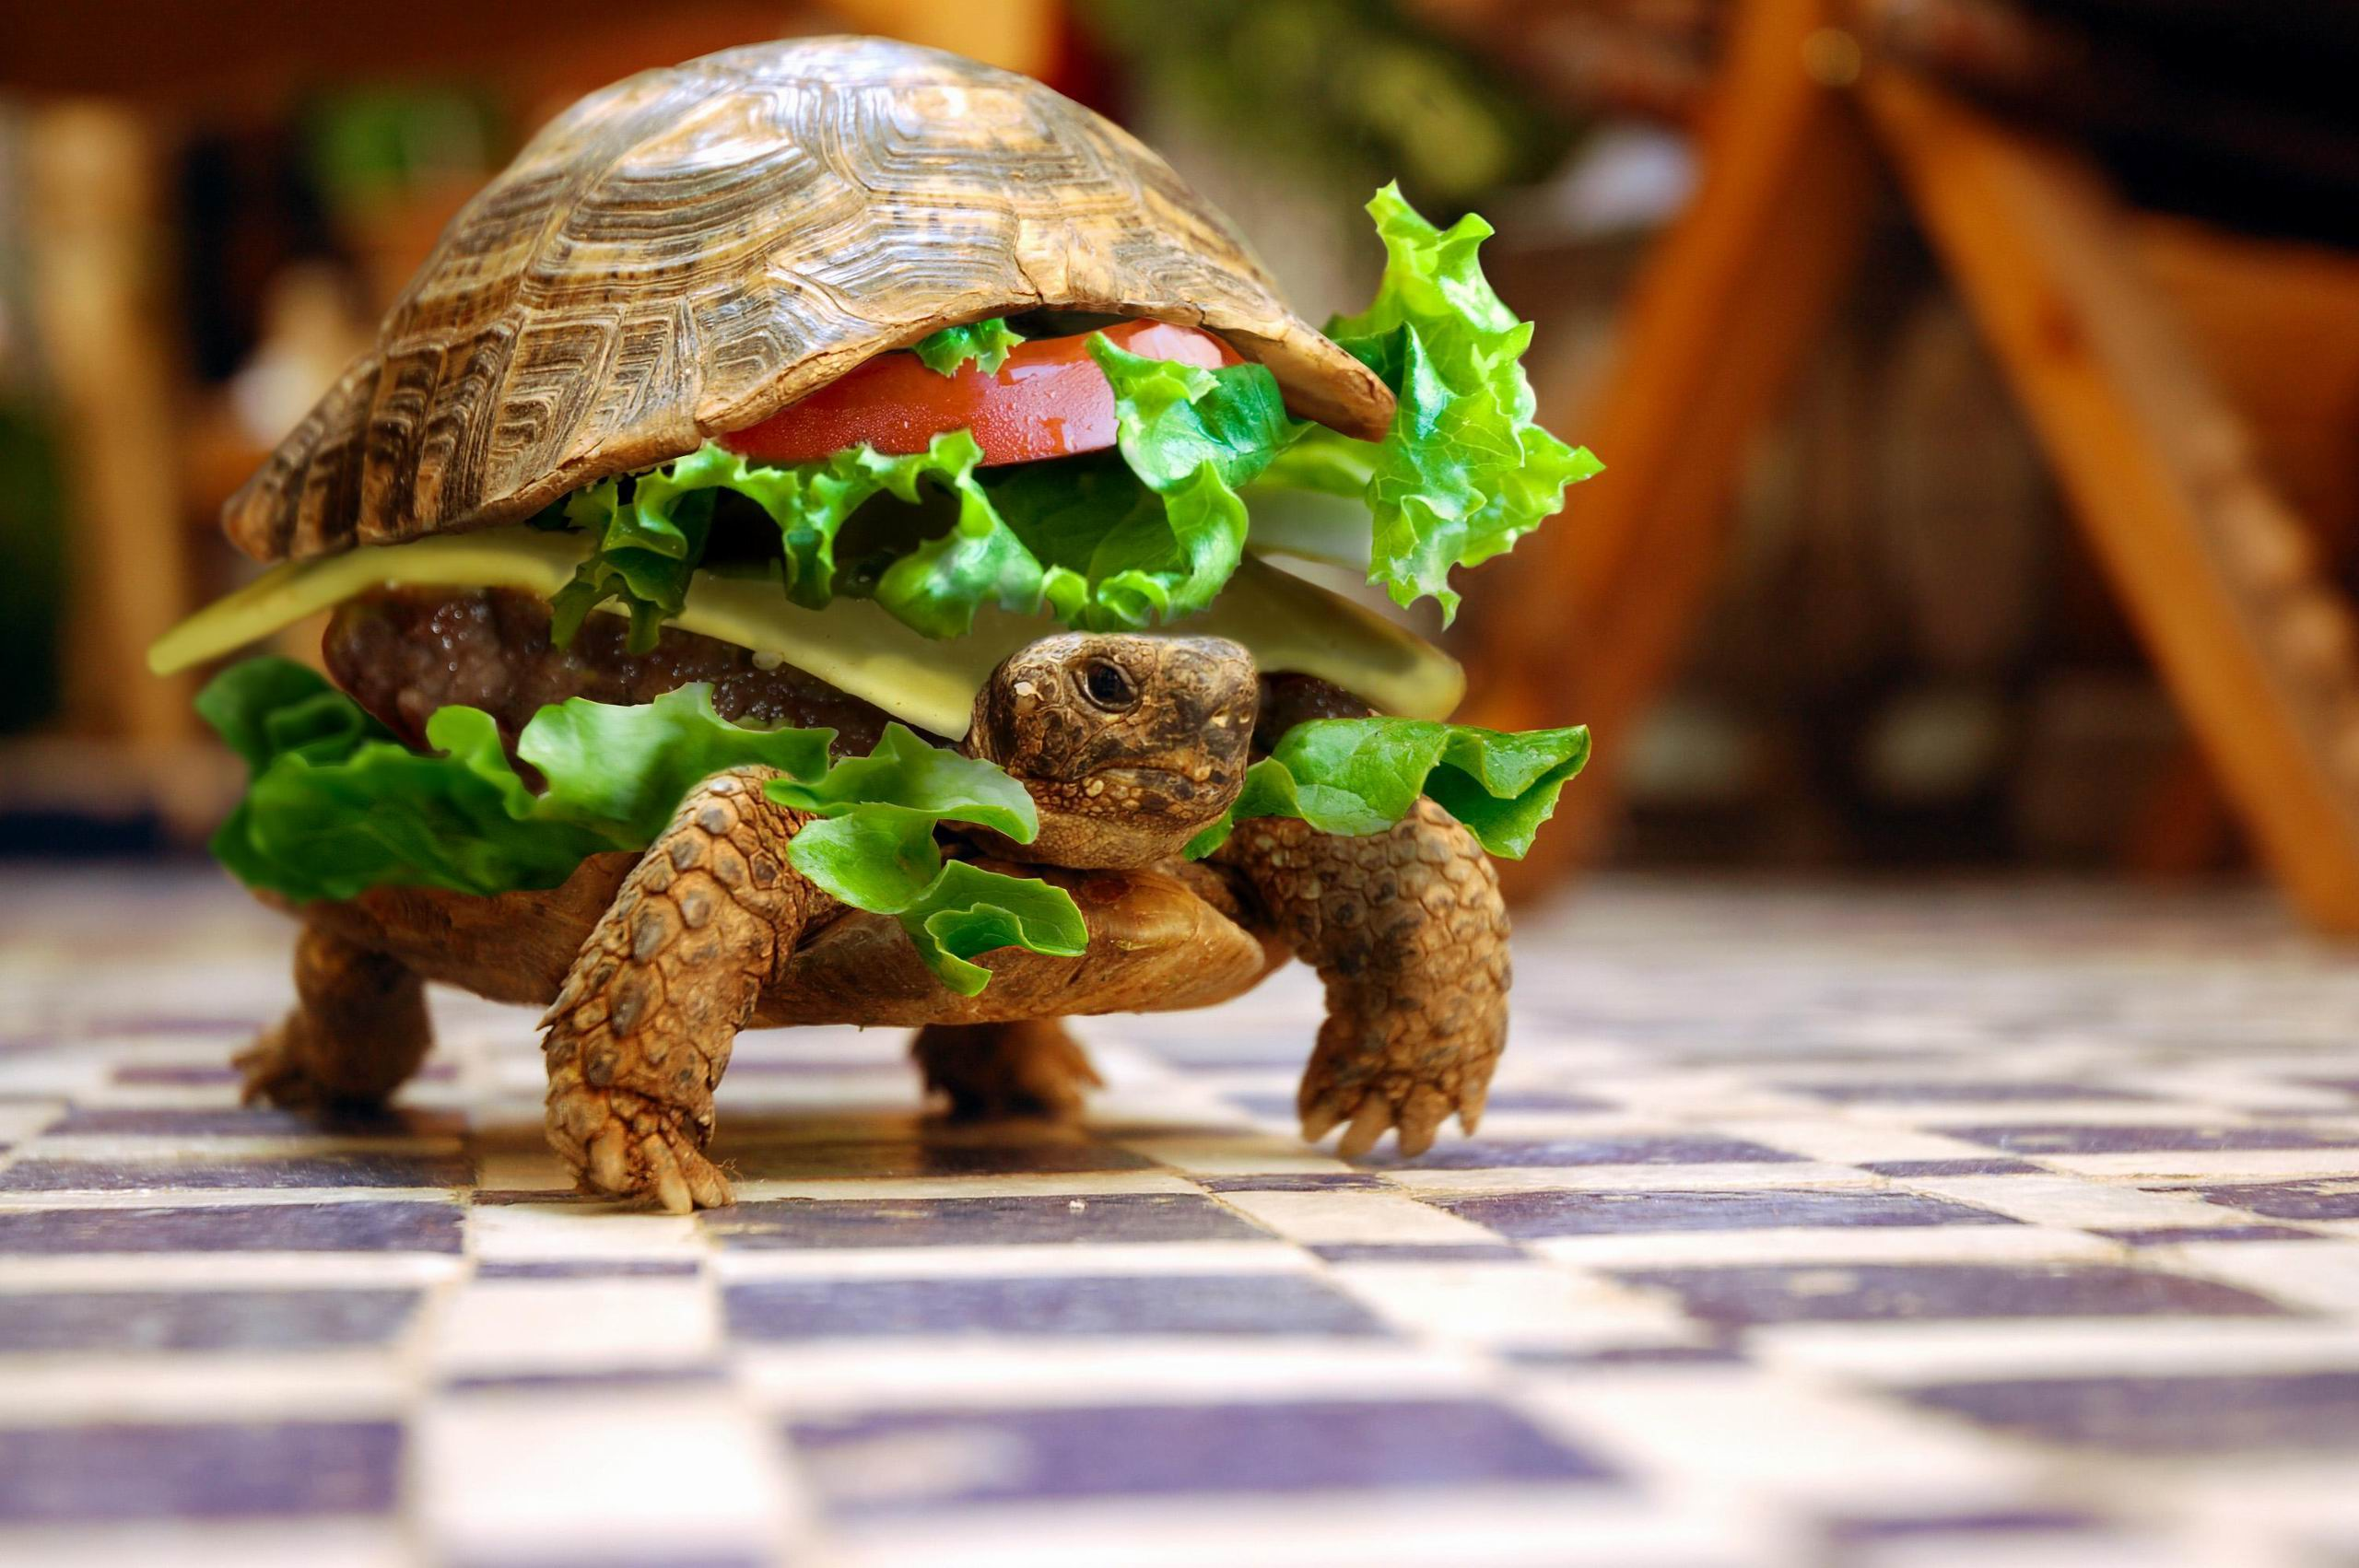
\includegraphics[width=\textwidth]{turtle-burger.jpg}
	\caption{A rare but delicious turtle burger in the wild.}
	\label{fig:turtleBurger}
\end{figure}

\section{Testing}
\label{sec:testing}

See Figure~\ref{fig:turtleBurger} for more details.

\section{Conclusion}
\label{sec:conclusion}

Conclusions are typically hard to write, so we'll save it for last. This is
once again just a placeholder because we haven't written this section yet.

\lipsum[1]

\clearpage % references should be on their own page

\printbibliography
\addcontentsline{toc}{section}{References}

\newpage

\appendices
\section{Proof of the First Zonklar Equation}
Appendix one text goes here.

\section{}
Appendix two text goes here.

\end{document}


